\documentclass{beamer}

\usetheme{Pittsburgh}
\usecolortheme{beaver}

\usepackage{dot2texi}
\usepackage{tikz}
\usetikzlibrary{shapes,arrows}
\usepackage{bookmark}
\usepackage{graphicx}
\usepackage{todonotes}

\mode<handout>{%
  \usepackage{pgfpages}
  \pgfpagesuselayout{resize to}[a4paper]
}

\title{Building a Web Search}
\author{Ross Fenning}
\institute{
  Senior Software Engineer
  \\Content Discovery
  \\Future Media
  \\BBC
}
\date{17 June, 2014}

\begin{document}

\begin{frame}[plain]
  \titlepage
\end{frame}

% Background
\begin{frame}
  \frametitle{About Me}
  \begin{itemize}
    \pause \item Senior Software Engineer
    \pause \item BBC Future Media
    \pause \item Content Discovery: Search
    \pause \item BBC Academy and University of Bradford, UK
    \pause \item Bournemouth University, UK and Lancaster University
    \pause \item School of Design Engineering \& Computing at Bournemouth University
  \end{itemize}
\end{frame}

\begin{frame}
  \frametitle{What is BBC Search?}
  \framesubtitle{i.e. What do I work on?}
  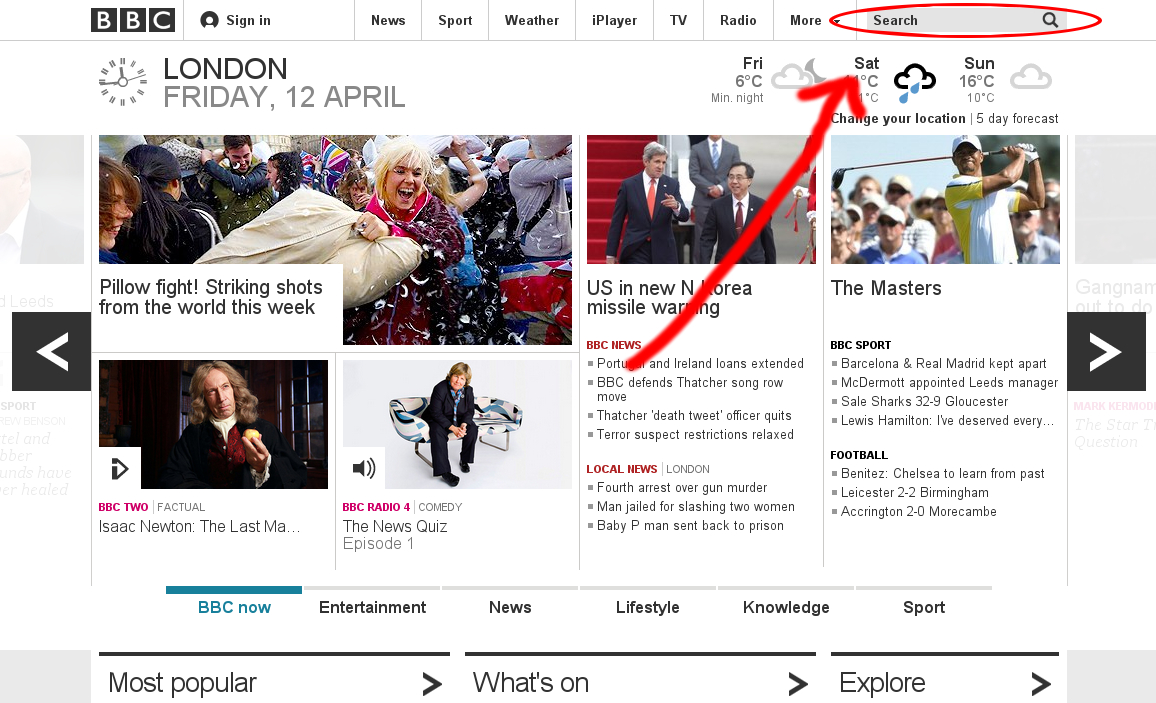
\includegraphics[width=\linewidth]{homepage.png}
\end{frame}

\begin{frame}
  \frametitle{Why BBC Search?}
  \framesubtitle{Isn't Google good enough?}
  \begin{itemize}
    \pause \item We can search the BBC via Google
    \pause \item What can the BBC offer that Google cannot?
  \end{itemize}
\end{frame}

% Design Goals
% Contextualisation of the problems space through SSM
% Extracting use cases
% Designing behaviour for indirect users
% Designing behaviour for direct users
% Domain modelling for search -- model business rules as per benefits shown in background, but also keep it generic
% Discussion and Analysis -- Use cases - More SSM needed?
% Discussion and Analysis -- Domain Model -- Polymorphism
% Discussion and Analysis -- Domain Model -- Duck Typing
% Discussion -- More SSM: 3 Es?
% Shortcomings -- Performance? NFRs?
% Shortcomings -- Agile?
% Validation?

\end{document}
